\section{The Proposed Method}
\label{sec:method}
This section introduces the detailed methodology of the our proposed W2CL framework, which mainly consists of two parts: domain knowledge extraction with ChatGPT and knowledge integration based on multi-task learning.
\subsection{Domain Knowledge Extraction with ChatGPT}
In the domain knowledge acquisition phase, we use ChatGPT as a knowledge extractor to extract the necessary domain knowledge for multi-task learning from a raw text corpus. This step can be divided into three stages, as shown in Figure~\ref{ke}.

In Step 1, we first use the Jieba tool to segment the raw text corpus and then compile a list of frequently occurring words. ChatGPT is then employed to filter out domain-specific vocabulary from this list, as illustrated in Figure~\ref{ke}.a, and the prompt1 shown in the Figure~\ref{ke}, "I currently have several terms. You will categorize all the terms I provide into levels of relevance: high, medium, and low. This relevance level pertains to a specific domain." Finally, extract the terms with high relevance to compile the final domain-specific vocabulary list.

In Step 2, ChatGPT is used to categorize the domain-specific vocabulary obtained in Step 1 into relevant categories within the domain, and the prompt2 is "Assume you are now an expert in the XX domain. Please classify the terms I provide within the subcategories of this domain.". This step allows us to obtain the initial version of domain-specific classification knowledge.

In Step 3, we manually consolidate all categories obtained in Step 2 to create a final comprehensive category list that covers all terms. Finally, we provide ChatGPT with this finalized category list to reclassify the vocabulary, producing the ultimate domain knowledge, and the prompt3 is "Assume you are an expert in the XX domain. I will provide you with several terms related to this domain, along with a list of categories: [Categories]. I need you to assign each of my terms to a category from the provided list. If a term cannot be assigned to any of the existing categories, please mark it as None. The required format for the response is 'Term: Category'.".

\begin{figure}[ht]
	\centering
	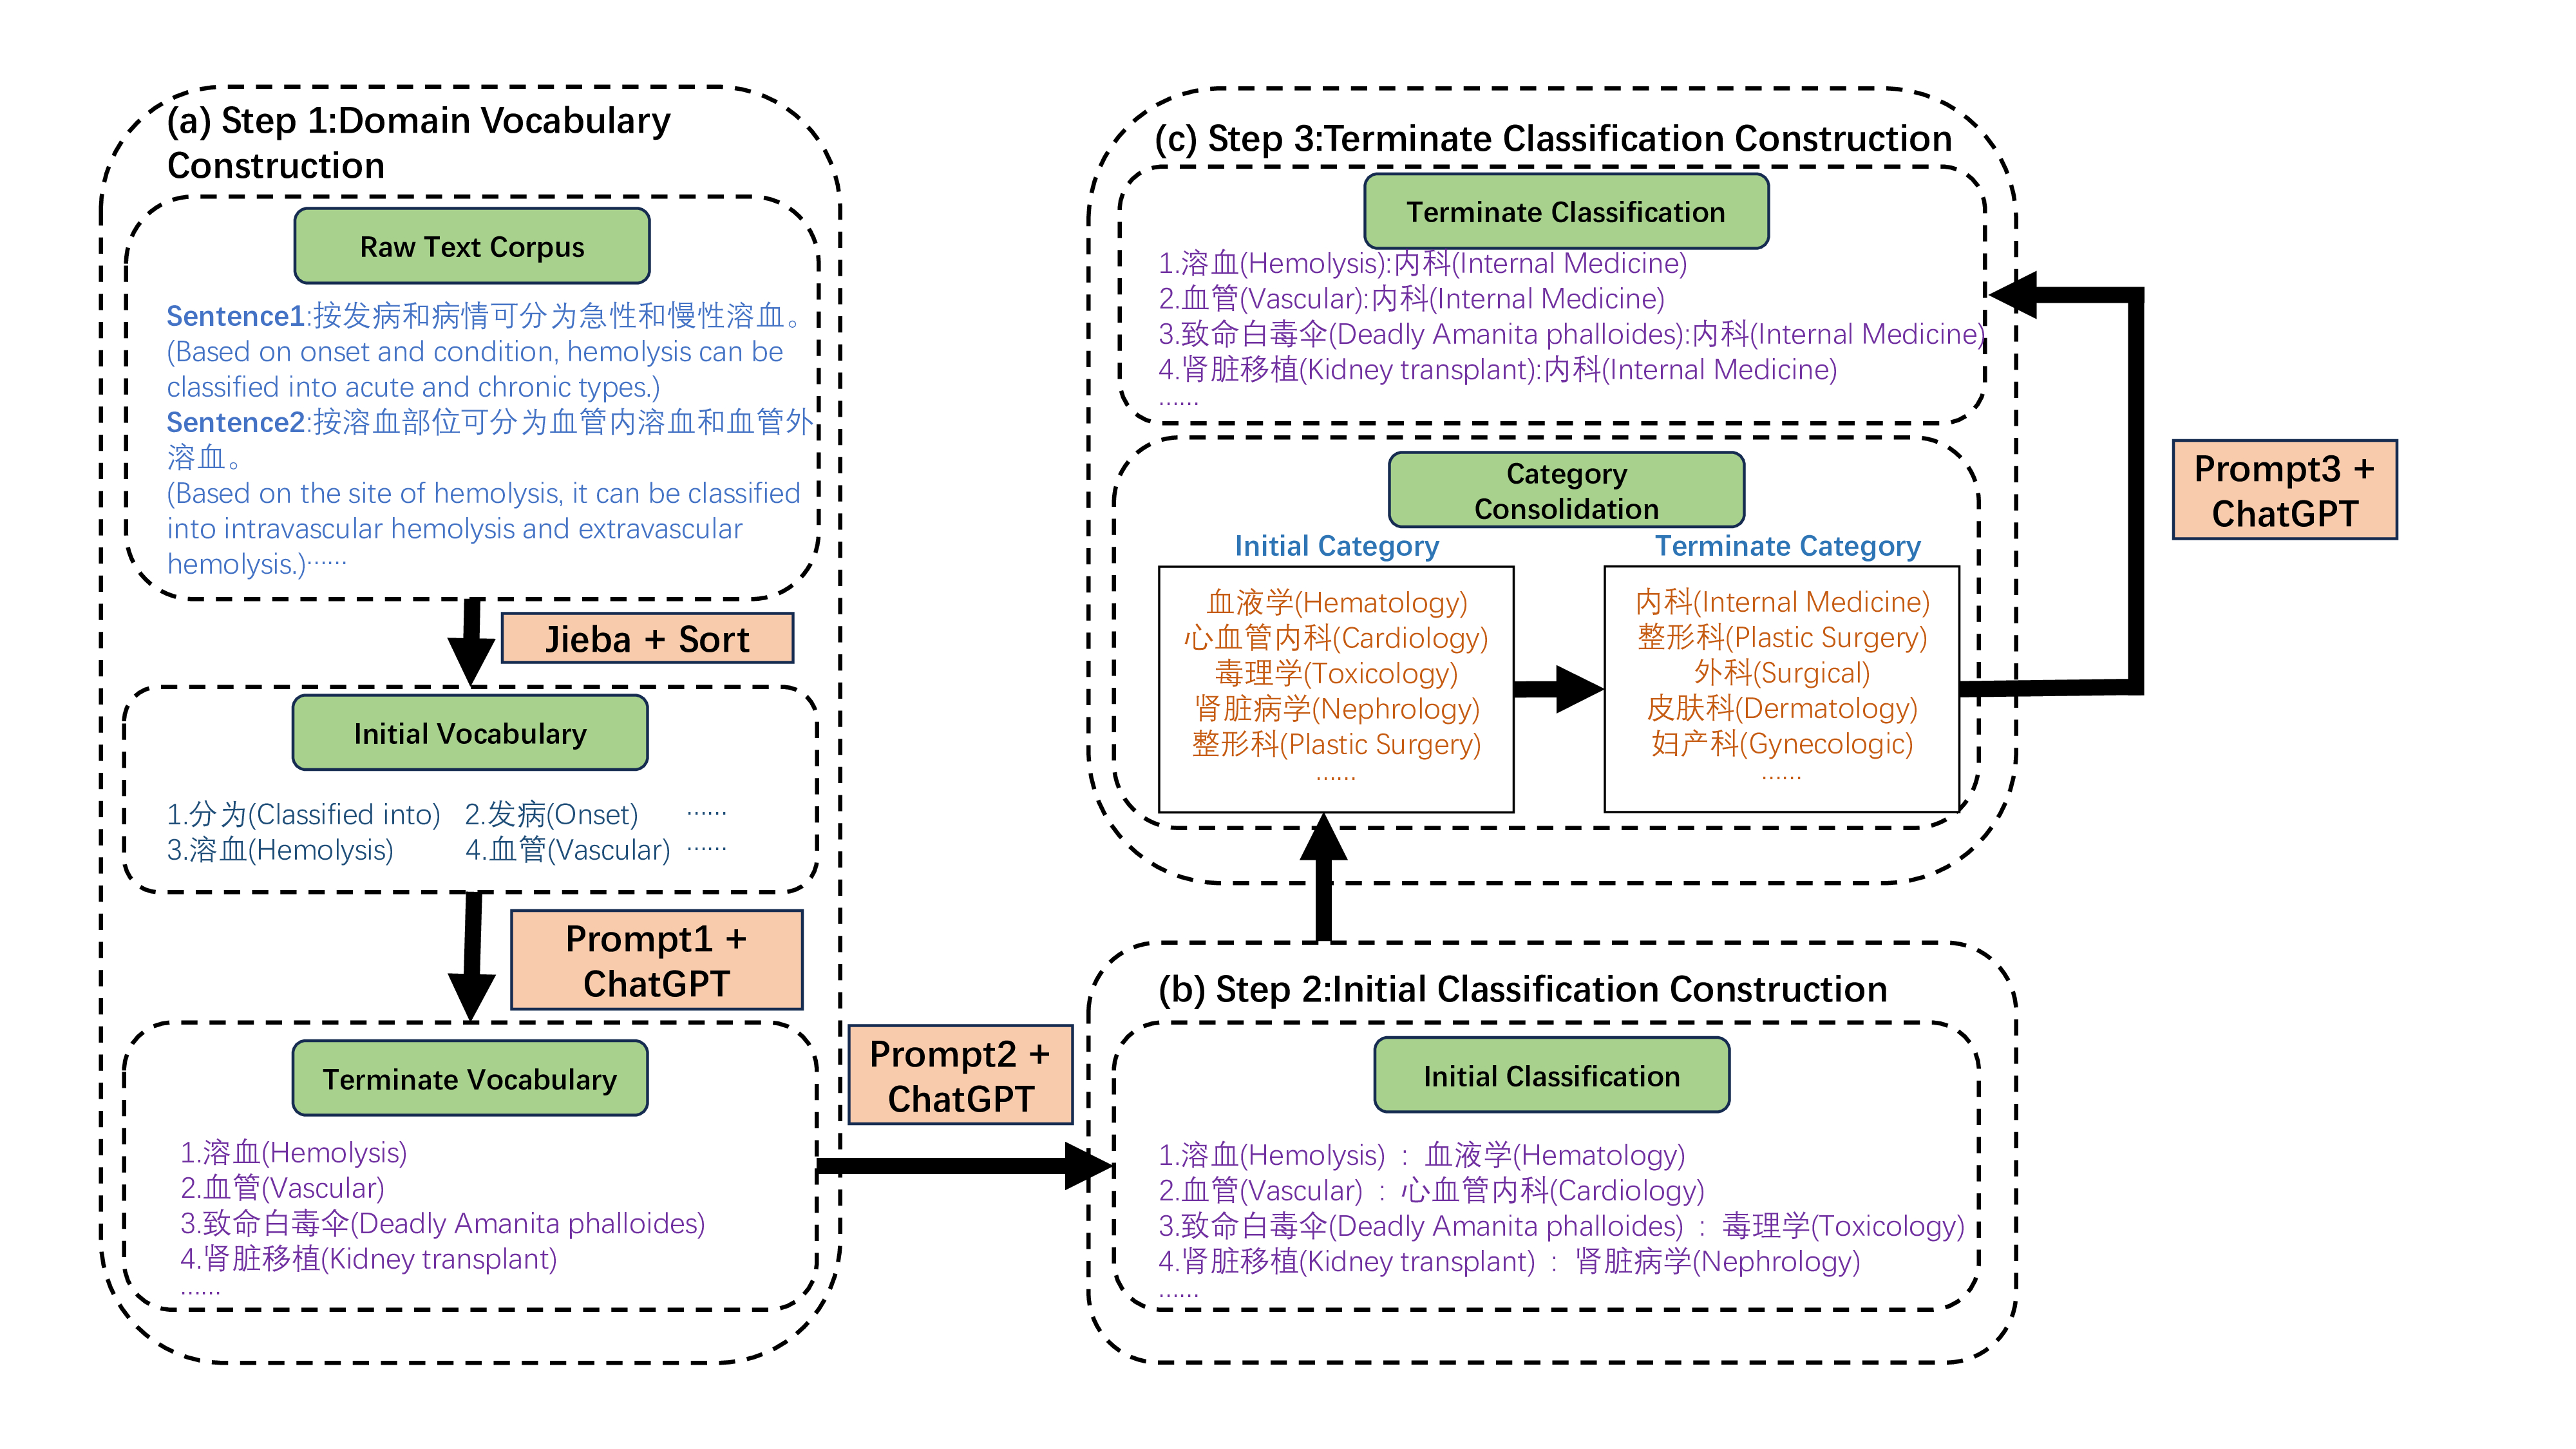
\includegraphics[width=1.0\textwidth]{ChatGPT} 
	\caption{Knowledge Extraciton Framework}
	\label{ke}
\end{figure}
\subsection{Domain Knowledge Intergration}
Our proposed knowledge intergration method is based on Whole Word Masking(WWM)\cite{macbert} and incorporates two additional training tasks: Word Classification and Contrastive Learning. The details about WWM will be introduced in the BASELINES section of Chapter 3. The following sections will introduce other two tasks individually.
\subsubsection{Word Classification.}
Given a sentence \{$x${\tiny 1}, $x${\tiny 2}, $x${\tiny 3}, [MASK], $x${\tiny 5}, [MASK],$x${\tiny 7}\} and a list of categories for the masked words \{$C${\tiny 1}, $C${\tiny 2}\}. Word Classification adds a classification layer to the original model architecture. The classification loss function is then computed as shown in Equation~\ref{tc}:
\begin{equation}
	\label{tc}
	L(\mathbf{y}, \mathbf{\hat{y}}) = - \sum_{i=1}^C \left( y_i \log(\hat{y}_i) + (1 - y_i) \log(1 - \hat{y}_i) \right)
\end{equation}
\begin{itemize}
	\item $\mathbf{y} = [y_1, y_2, \ldots, y_C]$: The multi-label binary vector of true labels, where $C$ is the number of classes. Each $y_i$ represents the true label for class $i$ ($1$ indicates the presence of the class, $0$ indicates the absence of the class).
	\item $\mathbf{\hat{y}} = [\hat{y}_1, \hat{y}_2, \ldots, \hat{y}_C]$: The predicted probability distribution vector from the model, where each $\hat{y}_i$ represents the predicted probability for class $i$, with values in the range $[0, 1]$.
	\item $L(\mathbf{y}, \mathbf{\hat{y}})$: The loss function value for the multi-label classification task.
	\item $C$: The total number of classes.
\end{itemize}
\subsubsection{Contrastive Learning.}
Given a sentence \{$x${\tiny 1}, $x${\tiny 2}, $x${\tiny 3}, [MASK], $x${\tiny 5}, [MASK],$x${\tiny 7}\}, and the actual words masked by [MASK] \{$x${\tiny 4}, $x${\tiny 6}\}.Our proposed contrastive learning method uses the actual word corresponding to the current [MASK] position as the positive sample for the current [MASK]. All the positive and negative samples of other [MASK] tokens from other sentences in the same batch are used as the negative samples for the current [MASK]. The specific calculation method is shown in Equation~\ref{cl}:
\begin{equation}
	\label{cl}
	L(\mathbf{t}, \mathbf{t'}) = -\frac{1}{N} \sum_{i=1}^{N} \log \frac{e^{sim(f(\mathbf{t}_i) \cdot f(\mathbf{t'}_i))/\tau}}{\sum_{j=1}^{N} e^{sim(f(\mathbf{t}_i) \cdot f(\mathbf{t'}_j))/\tau}}
\end{equation}
\begin{itemize}
	\item $\mathbf{t} = [t_1, t_2, \ldots, t_N]$: $N$ is the number of [MASK] in one batch. Each $f$($t_i$) represents the representation of $i_{st}$ [MASK] token in the batch.
	\item $\mathbf{t'} = [t'_1, t'_2, \ldots, t'_N]$: $f$($t'_i$) represents the representation of the true label $t'_i$ corresponding to the $i_{st}$ [MASK] token, which is the positive sample for $f$($t_i$).
	\item $L(\mathbf{t}, \mathbf{t'})$: The loss function value for the contrastive learning task.
	\item \(sim(\mathbf{h1} \cdot \mathbf{h2})\): \(sim(\mathbf{h1} \cdot \mathbf{h2})\) is the cosine similarity \(\tfrac{\mathbf{h1}^T\mathbf{h2}}{\lVert \mathbf{h1} \rVert \cdot \lVert \mathbf{h2} \rVert}\).
	\item \(\tau\): is a temperature hyperparameter, with a default value of 0.01.
\end{itemize}
\subsubsection{Training Framework.}
The overall training objective comprises three terms:
\begin{equation}
	\label{allloss}
	L_{overall} = L_{WWM} + L_{WC} + L_{CL} 
\end{equation}
where \(L_{WWM}\) is the loss of the WWM task,\(L_{WC}\) is calculated by equation~\ref{tc},and \(L_{CL}\) is calculated by equation~\ref{cl}.

\begin{figure}[ht]
	\centering
	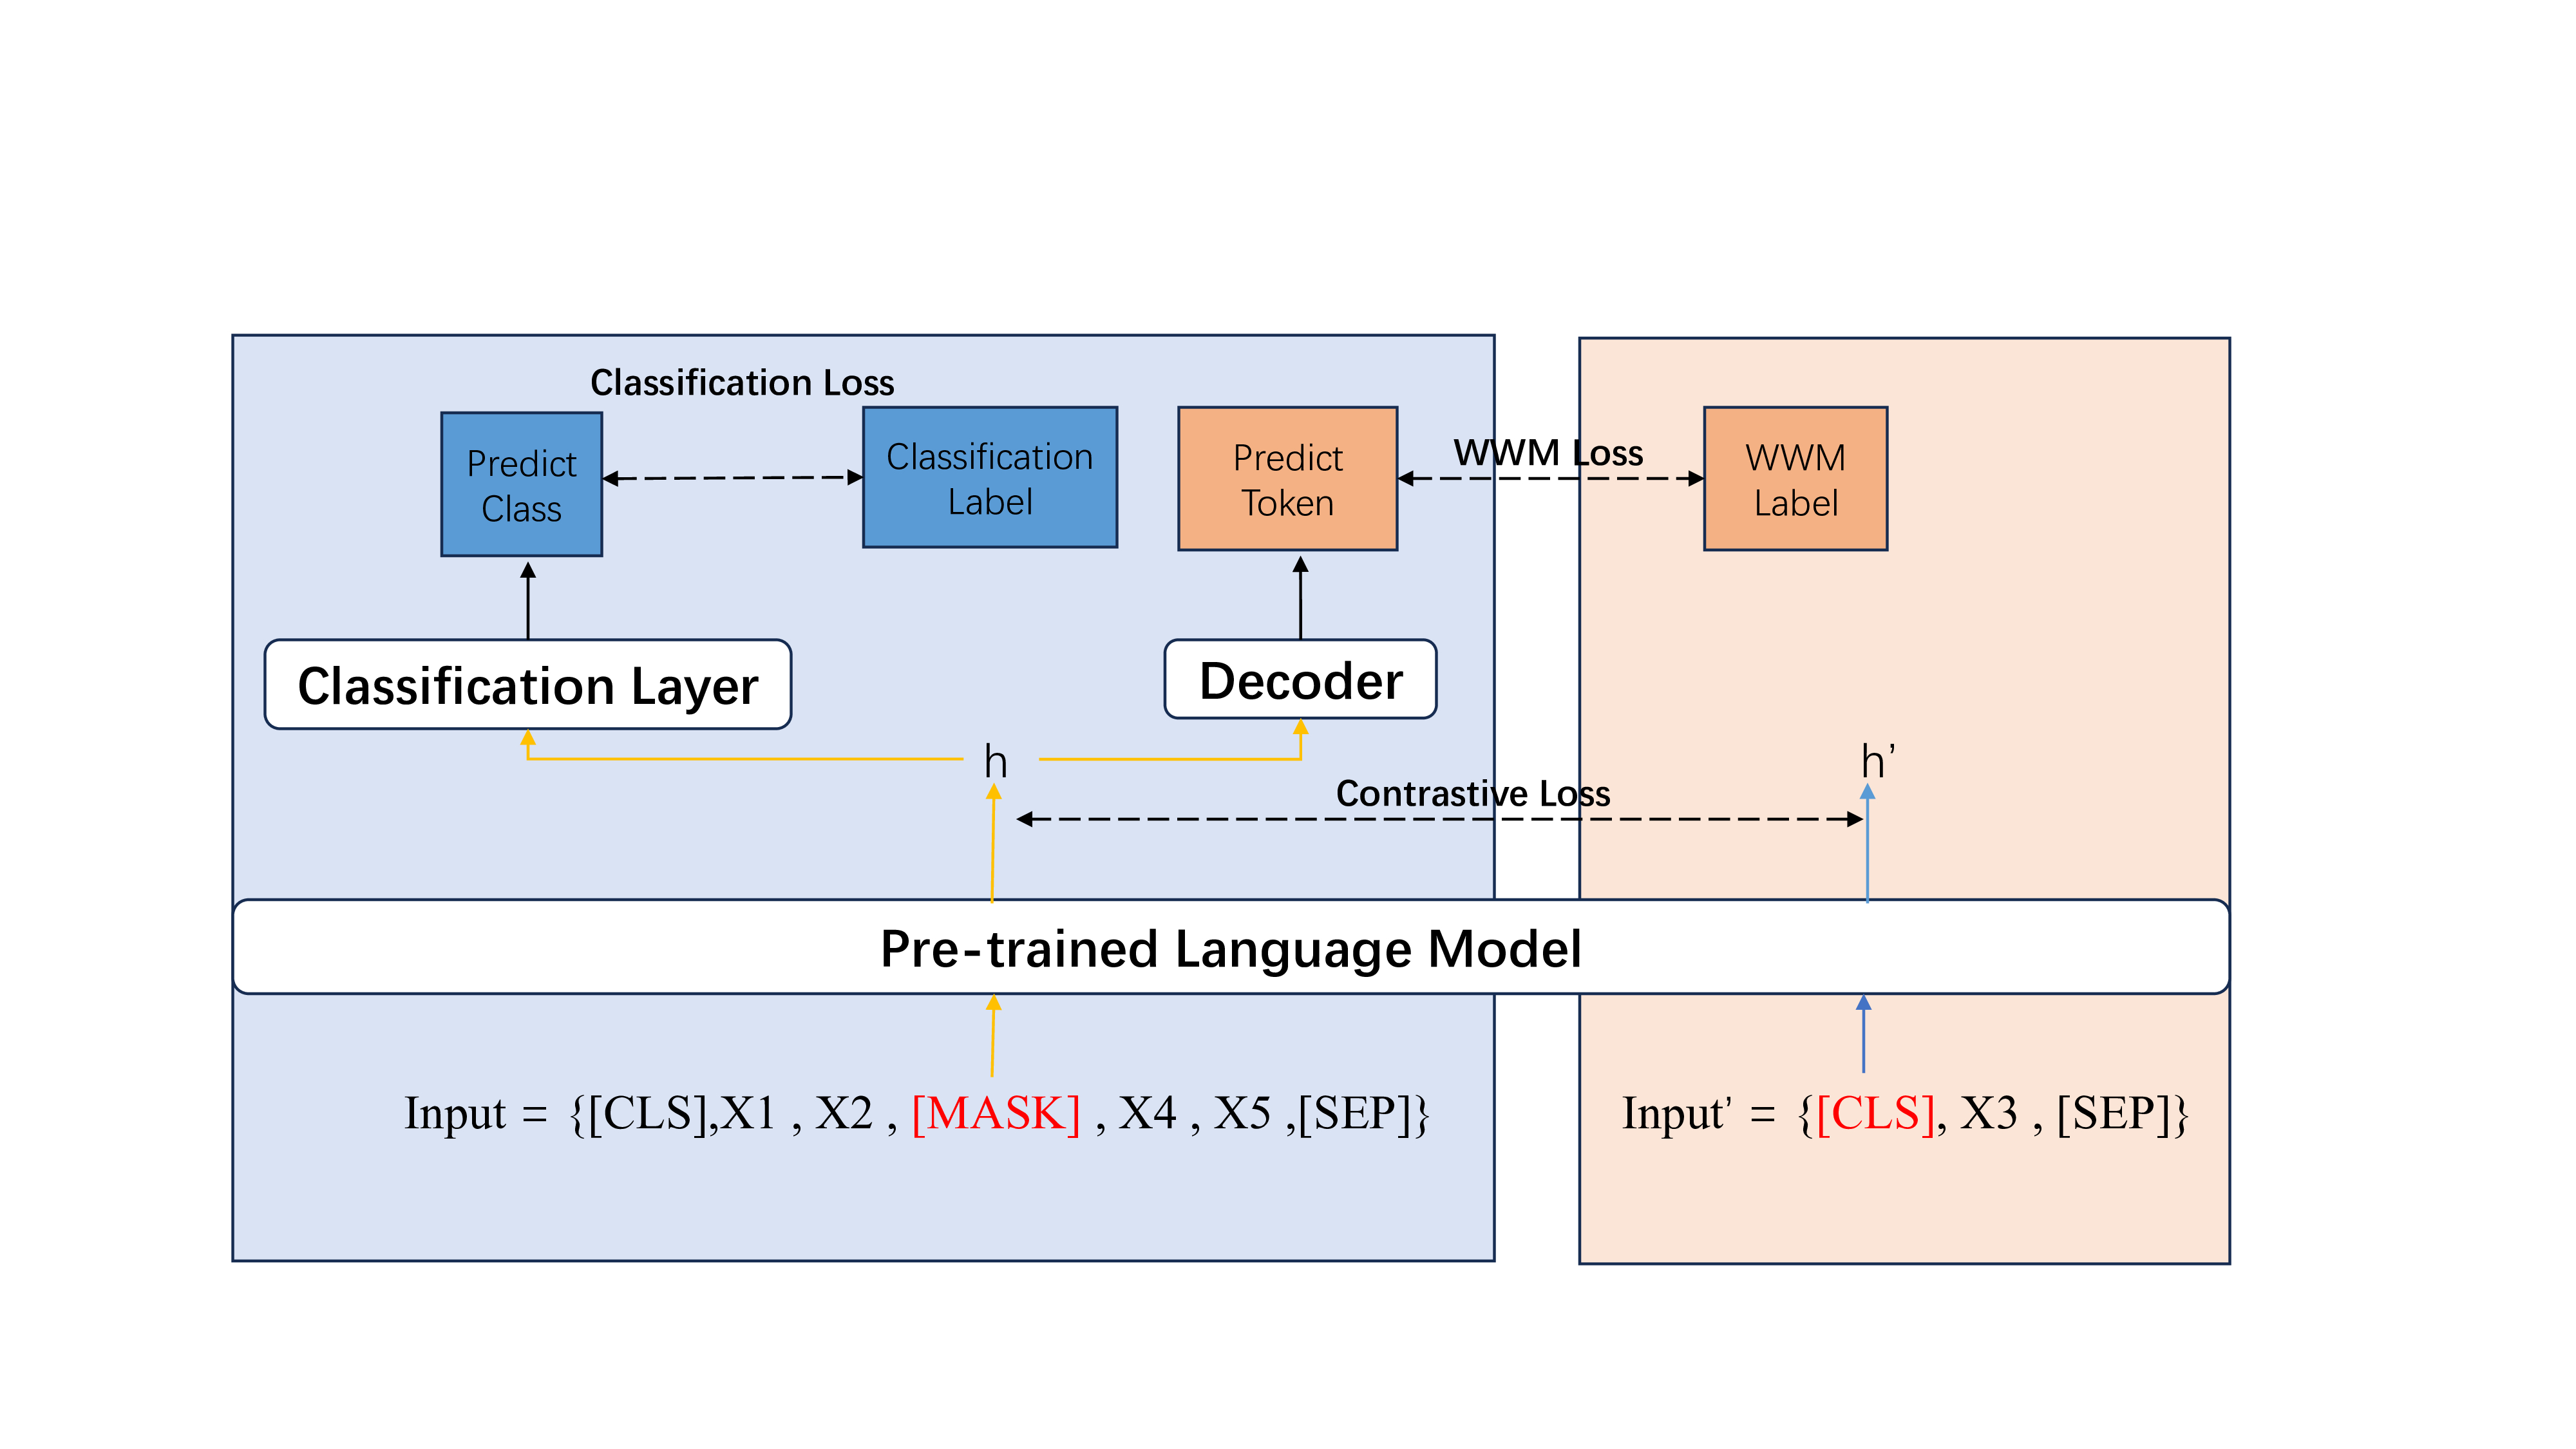
\includegraphics[width=1.0\textwidth]{train_framework} 
	\caption{Training Framework}
	\label{train}
\end{figure}

The training framework is depicted in Figure~\ref{train}. Firstly, we obtain the loss(\(L_{WWM}\)) for the WWM task, which aims to help the model learn the meanings, usage, and contextual relationships of vocabulary, facilitating the model's adaptation to the specific domain context. Secondly, the loss(\(L_{CL}\)) from contrastive learning can assist the model in gradually learning the semantic similarity and contextual relevance between words during the training process, thereby enhancing its ability to understand text. Finally, the loss(\(L_{WC}\)) from word classification provides additional contextual understanding and domain knowledge, thereby improving the model's ability to differentiate between different classes within the specific domain.


